%%%%%%%%%%%%%%%%%%%%%%%%%%%%%%%%%%%%%%%%%%%%%%%%%%%%%%%%%%%%%%%%%%%%%%%%%%
%
%    JWST_sci_template.tex  (use only for JWST General Observer and Archival Research proposals)
%
%
%
%    JAMES WEBB SPACE TELESCOPE
%    OBSERVING PROPOSAL TEMPLATE
%    FOR CYCLE 1 (2017)
%
%    Version 1.0 September 2017.
%
%    Guidelines and assistance
%    =========================
%     Cycle 1 Announcement Web Page:
%
%         https://jwst-docs.stsci.edu/display/JSP/JWST+Cycle+1+Proposal+Opportunities
%
%    Please contact the JWST Help Desk if you need assistance with any
%    aspect of your proposal:
%    	    http://jwsthelp.stsci.edu
%
%
%
%%%%%%%%%%%%%%%%%%%%%%%%%%%%%%%%%%%%%%%%%%%%%%%%%%%%%%%%%%%%%%%%%%%%%%%%%%%

% The template begins here. Please do not modify the font size from 12 point.

\documentclass[12pt]{article}
\usepackage{jwstproposaltemplate}
\usepackage{hyperref}
\usepackage{graphicx}
\usepackage{floatrow}
\usepackage{sidecap}
\sidecaptionvpos{figure}{t}



\usepackage{natbib}
\bibliographystyle{mnras}

% \usepackage[]{biblatex}
% \addbibresource{WAFLS.bib}
% \addbibresource{WAFLS_quiescent.bib}

\setlength{\textfloatsep}{5pt}
\usepackage{color}

\newcommand{\todo}[1]{\textbf{**TODO: \textcolor{red}{#1}**}}


\begin{document}

%   1. SCIENTIFIC JUSTIFICATION
%       (see https://jwst-docs.stsci.edu/jwst-opportunities-and-policies/jwst-call-for-proposals-for-cycle-1/jwst-cycle-1-proposal-preparation)
%
%






\todo{Abstract. Delete later.}

We propose WAFLS - the Wide Area First Light Survey. WAFLS is a pure-parallel programme designed to build up a large ($\sim 1350$arcmin$^2$) area of medium-depth (F200W=$28.5$) 6-band near-infrared ($1-5\mu$m) imaging with NIRCam. WAFLS complements planned GTO and ERS programmes by obtaining shallower imaging over an area $4-5\times$ larger (comparable to {\it HST}'s CANDELS survey), separated into $\sim$150 independent pointings, minimising the effect of cosmic variance. The primary scientific motivation of WAFLS is the identification and characterisation of the $L^{\star}$ galaxies at $9<z<11$ including placing strong constraints on the bright-end of the luminosity function. The multi-wavelength observations observations obtained by WAFLS will enable the accurate measurement of key physical properties of these galaxies including the star formation rate, morphologies, dust attenuation, and stellar masses. The sources identified by WAFLS will be more amenable to multi-wavelength follow-up with other facilities. The secondary motivation is the selection of high-$z$ passive (i.e. non star-forming) galaxy candidates and the analysis of their abundance at $3<z<6$. The large area observed by WAFLS will be key to identify such sources, rare yet crucial to constrain the physical mechanisms responsible for their rapid assembly and efficient star formation suppression in the early Universe.  Compared to JADES (CEERS), WAFLS will include ~5x (~10x) more quiescent galaxies at $z>3$.  




\clearpage

\justification          % Do not delete this command.


The advent of the {\it James Webb Space Telescope} brings two major advances -- light-gathering power and sensitivity to $\lambda >$ 2$\mu$m.  These will lead to transformative advances in a number of fields, including \emph{Webb}'s two primary science goals: First Light and Galaxy Assembly.  Of the many major questions which exist in these areas, two stand out.  1) What is the abundance of bright galaxies at $z >$ 9, and what does this tell us about how stars form at early times?  2) When do the first quiescent galaxies form, and how do they quench their star formation?  Answers to both require {\it Webb}'s light gathering power and red sensitivity.  However, these sources are intrinsically rare, and are not randomly distributed due to fluctuations in the large-scale dark matter density field \citep[e.g.][]{2008ApJ...676..767T, 2020MNRAS.496..754B, 2020MNRAS.499.2401T}.  Thus planned Cycle 1 surveys such as the Cosmic Evolution Early Release Science (CEERS) and the JWST Advanced Deep Survey (JADES) GTO program will not only be unable to robustly quantify the abundance of both types of galaxies but also adversely affected by cosmic variance resulting in weaker constraints on the luminosity function \cite{2020MNRAS.499.2401T}.  

We propose to overcome this barrier \emph{virtually for free} with a pure parallel survey.
\emph{Webb}, like \emph{Hubble}, has the ability for most observing modes to utilise a second instrument in parallel. By virtue of the nature of piggybacking on to a diverse set of primary observations spread across the sky, parallel opportunity targets have minimum cosmic variance resulting in smaller uncertainties on the number density. Pure parallel imaging programs on \emph{Hubble}, including HIPPIES \citep{2011ApJ...728L..22Y} and BoRG \citep{2011ApJ...727L..39T}, provided useful constraints on bright-end of the $z>7$ luminosity function \citep[e.g][]{2014ApJ...786...57S, 2016ApJ...817..120C, 2016ApJ...827...76B, 2020ApJ...891..146R, 2020arXiv201015637M}, complementing deeper surveys such as CANDELS and the HUDF. With these considerations in mind we propose the \textbf{Wide Area First Light Survey (WAFLS)}, a pure-parallel programme to obtain wide-area public multi-band near-IR ($\sim 1-5\mu m$) imaging using NIRCam over multiple independent sight-lines.  WAFLS will probe an area almost 5$\times$ larger than planned GTO/ERS surveys, spread out over $\sim$140 independent pointings, resulting in galaxy abundances with minimal cosmic variance uncertainties.  Our results, in combination with theoretical models, will make important progress in understanding the physical processes responsible for driving both star formation and quenching in the early Universe. 

\noindent
\textbf{The primary scientific objectives of WAFLS are:}
\vspace{-1mm}
\begin{enumerate}
\item The robust identification of tens of bright (F200W$<28$) galaxies across the early EoR ($9<z<11$) amenable to multi-wavelength follow-up.
\item Cosmic variance minimised constraints on the $9<z<11$ luminosity function around $L^{\star}$.
\item The measurement of the physical properties of $9<z<11$ galaxies including their star formation rates, stellar masses, dust attenuation, and morphologies. 
\item Constraints on the space density and properties of quiescent galaxies at $z>3$ including the first useful constraints at $z>5$.
\end{enumerate}

While focused on the distant Universe WAFLS will provide an invaluable immediately public legacy resource for answering a range of other science questions. WAFLS will, for example, enable the discovery and typing of low-mass stars and sub-stellar objects throughout the disk and halo of the Milky Way. When combined with optical observations WAFLS will enable the measurement of accurate stellar masses and star formation rates across cosmic history, reaching down to $M_{\star}\sim 10^{8}\,{\rm M_{\odot}}$ at $z=2$.


\subsection*{Constraints on the UV Luminosity Function Across the Epoch of Reionisation and Beyond}\label{sec:UVLF}

The observed luminosity function of galaxies encodes both the  detailed physics of star formation in addition to the effect of dust attenuation. From a theory perspective both of these are sufficiently uncertain, particularly in the early Universe, that different modelling approaches, despite yielding similar results at low-redshift, diverge at high-redshift. This is demonstrated in Figure \ref{fig:CN_models} where we show the expected cumulative number of galaxies expected in WAFLS for a range of models. This wide variation demonstrates that the study of galaxies during this epoch has potential to inform our understanding of galaxy formation and evolution in the early Universe.

\begin{SCfigure}
    \includegraphics[width=0.6\textwidth]{figs/CN_models_WAFLS.pdf}
      \caption{\protect\rule{0ex}{5ex} The cumulative number of sources predicted to observeable by WAFLS by a range of models. These include empirical extrapolations (Finkelstein+2016), semi-empirical models (Mason+2015, Williams+2018), semi-analytical models (Yung+2018), and hydrodynamical simulations (Wilkins+2017; Ma+2019; Vijayan+2020).}
      \vspace{-10mm}
\end{SCfigure}


\todo{What has been done and how will WAFLS change things?}
\todo{Should we mention Hubble constraints? - I feel we're not fighting Hubble but other Webb programmes.}

While the planned GTO/ERS programmes will begin the process of obtaining stronger constraints at $z>9$ the relatively small areas probed by these programs limits the number of bright galaxies. This limits our ability to constrain the bright-end of the LF, critical to characterise its overall shape. Compounding the small number of sources is the fact that these programmes, as predominantly contiguous surveys, will suffer from cosmic variance increasing the uncertainty on the number of galaxies by $\approx 1.5-2\times$ compared to the statistical uncertainty alone\cite{2020MNRAS.499.2401T}\cite{2020MNRAS.496..754B}\cite{2008ApJ...676..767T}. 

\begin{SCfigure}
    \includegraphics[width=0.6\textwidth]{figs/CV.pdf}
      \caption{\protect\rule{0ex}{5ex} The predicted number of sources at $9<z<10$ as a function of F277W in CEERS, JADES, and WAFLS. The upper-panel shows the total variance $\sigma^2$ compared to the expected statistical variance $N$. This demonstrates that WAFLS suffers from minimal cosmic variance while both JADES and CEERS suffer a factor of $2-4$ larger variance than naively expected for the given number of galaxies.}
      \label{fig:CV}
      \vspace{-5mm}
\end{SCfigure}

The wide area and pure parallel nature of WAFLS overcomes these issues. The WAFLS strategy is tuned to probe $M^{\star}$ ($M_{1500}=-20\ -\ 21$) galaxies at $9<z<11$ yielding roughly uniform number of galaxies per mag at F277W$27.5-29.5$ ($-21<M_{1500}<-18$) when combined with JADES and CEERS. Figure \ref{fig:CV} shows both the predicted number of sources and the total variance compared to the expected statistical variance for WAFLS, CEERS, and JADES. WAFLS yields not only $3\times$ as many galaxies as JADES+CEERS at F277W$<28.25$ but the resulting total uncertainty is virtually cosmic variance mitigated resulting in an even stronger gain. In Figure \ref{fig:LF} we show the resulting constraints on the $9.5<z<10.5$ LF from CEERS+JADES both with and without WAFLS. This highlights the strong improvement, particularly at $-21<M_{1500}<-20$ where $M^{\star}$ is expected to lie. The addition of WAFLS provides roughly uniform sampling of the LF over and reduces the uncertainty on both the parameters by around a factor of $2-3$. As shown in the right-hand panel WAFLS, when combined with CEERS and JADES, is able to discriminate between many current models. 

\begin{figure}[h!]
    \centering
    \includegraphics[width=0.5\textwidth]{figs/LF_10_combined.pdf}
    \includegraphics[width=0.45\textwidth]{figs/fitLF_alpha_phi.pdf}
    \vspace{-5mm}
    \caption{Expected constraints on the $9.5<z<10.5$ luminosity function, assuming the Mason+2015 model, for WAFLS, CEERS, and JADES. Uncertainties are corrected for the effects of cosmic variance. Sources are included if they are brighter than the 10$\sigma$ point-source limit. The right hand panel shows the joint constraints on the faint-end slope $\alpha$ and the number density at $M_{1500}=-20.5$ both using WAFLS and without WAFLS (JADES+CEERS). The right hand panel also shows various empirical and model predictions.}
    \label{fig:LF}
\end{figure}

\subsection*{The Physical Properties of Galaxies in the EoR}\label{sec:properties}

\begin{SCfigure}
    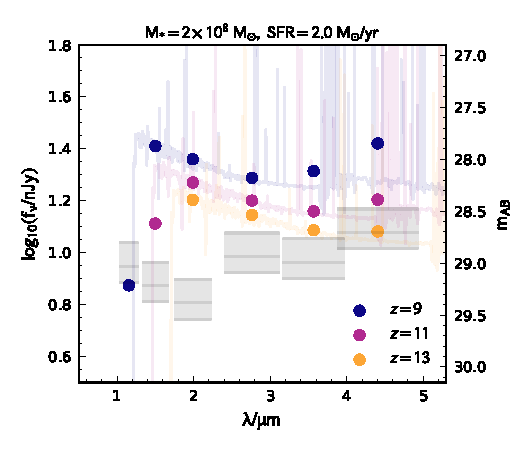
\includegraphics[width=0.6\textwidth]{figs/SED.pdf}
      \caption{\protect\rule{0ex}{10ex} The spectra and NIRCam fluxes of $5\times 10^{8}\ {\rm M_{\odot}}$ star forming galaxies at $z=9$ and $z=11$. Circled points denote a restricted 4 filter strategy; although this can be used to identify $z>9$ galaxies it neither enables the consistent measurement of the UV continuum slope $\beta$ across the target redshift range or allows constraints on the strength of the Balmer/$4000{\rm\AA}$ range.}
      \label{fig:SED}
\end{SCfigure}

The shape of the rest-frame UV continuum emission (the UV continuum slope, or $\beta$ where $f_{\lambda}\propto\lambda^{\beta}$) is a powerful probe of the physical properties of star forming galaxies. These properties include dust attenuation, stellar metallicity, star formation history, and ionising photon escape fraction \cite{2013MNRAS.430.2885W}. Particularly blue slopes ($\beta\simeq -3$) are indicative of the presence a young, low-metallicity, stellar population. While measurements of $\beta$ are available at $z\approx 7$ with {\em Hubble} these are typically measured with only a single colour over a relatively short wavelength baseline leading to large uncertainties and biases. While it is possible to measure $\beta$'s at $z\approx 10$ by combining {\em Hubble} and {\em Spitzer} observations \cite{2016MNRAS.455..659W}, these rely on the significantly shallower {\em Spitzer} imaging and have larger uncertainties. The 6 filter strategy of WAFLS (see Figure \ref{fig:SED}) will enable the consistent measurement of $\beta$ at $9<z<11$ over the entire rest-frame UV continuum. As demonstrated using simulated galaxies in Figure \ref{fig:beta}, when combined with F444W the degeneracy of $\beta$ with these physical properties can be broken allowing the measurement of stellar masses, specific star formation rates, and dust attenuation. Measuring the dust attenuation not only allows us to account for obscured star formation but will also help constrain the mechanism(s) responsible for the assembly of the large observed reservoirs of dust in the early Universe.



\begin{figure}[h!]
    \centering
    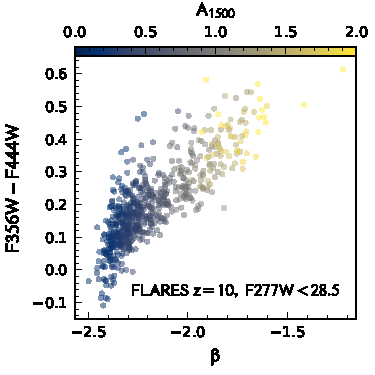
\includegraphics[width=0.3\textwidth]{figs/beta_A1500.pdf}
    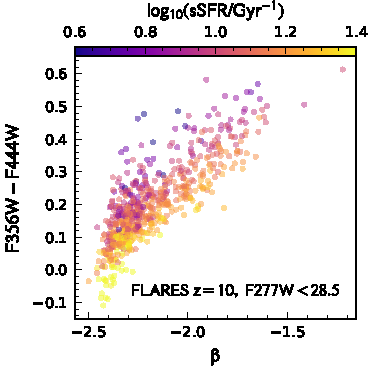
\includegraphics[width=0.3\textwidth]{figs/beta_sSFR.pdf}
    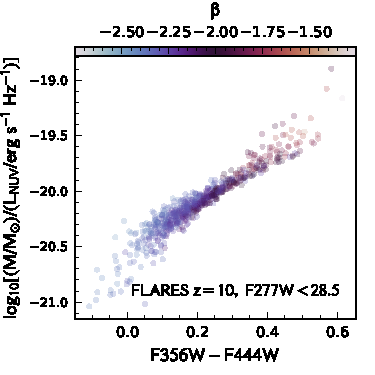
\includegraphics[width=0.3\textwidth]{figs/C_beta_MTOL.pdf}
    \caption{\emph{Left (middle):} The relationship between $\beta$ and F356W-F444W for simulated galaxies at $z=10$ colour-coded by $A_{1500}$ (sSFR) predicted by the FLARES simulation (Lovell+2020; Vijayan+2020). At these redshifts $\beta$ is strongly correlated with dust attenuation while at fixed $\beta$ the specific SFR is correlated with F356W-F444W. \emph{Right:} The relationship between F356W-F444W and the rest-frame NUV mass-to-light ratio. This demonstrates that stellar masses can be accurately determined using this single colour.}
    \label{fig:beta}
\end{figure}


% Morphologies

The morphologies and sizes of galaxies encode information about their structural properties and formation histories and are key observables that can be compared to galaxy formation models. Morphologies are also an important assumption used in the measurement of the luminosity function (reference) and only by simultaneously modelling the morphologies, redshifts, and fluxes is it possible to self-consistently measure the luminosity function and its uncertainties. Leveraging NIRCam's resolution WAFLS will provide sizes and morphologies of $9<z<11$ galaxies across the rest-frame UV ($0.1-0.4\mu$m). \todo{Maybe we should make a plot comparing the predicted size of galaxies to the NIRCam pixel scale and PSF?}


\subsection*{The Emergence of the First Quiescent Galaxies, $3<z<6$}

Over the last 10-15 years, passive galaxies have been identified at progressively higher redshift \citep[e.g.][]{cimatti04, saracco05, labbe05, kriek06, fontana09, straatman14, nayyeri14, schreiber18, merlin18, merlin19, carnall20, shahidi20}.
The existence of massive galaxies with suppressed levels of SF challenges theoretical models, which are still unable to correctly reproduce their abundance \citep[e.g.][, Santini et al. 2020]{vogelsberger14, feldmann16, merlin19, girelli19, shahidi20}. These galaxies result from complex physical processes that are still poorly understood. They have indeed assembled a large amount of mass over short timescales, implying very intense SF activity in their past \citep[e.g][]{merlin19}, and experienced likewise efficient mechanisms to prevent them forming new stars over the last 11 Gyr (at least). Understanding the evolution of early passive galaxies is fundamental to reach a global comprehension of galaxy evolution.

Early passive galaxies are also extremely challenging from an observational point of view. Current studies are limited by two main issues: selection accuracy and scarcity of candidates. 
The reliability of the selection is significantly hampered by the faintness of the candidates in the rest-frame UV. Their selection indeed strictly depends on the availability of deep NIR photometry. While photometric selection techniques based on SED fitting have been proved to be accurate enough, at least statistically \citep{santini19} and for the few cases where spectroscopic observations were available \citep{carnall20}),\citet{merlin18} has shown that \emph{Webb} data will allow a much cleaner selection. Moreover, while WFC3 observations of the CANDELS survey have enabled the assembly of the first statistically meaningful samples at $z>3$ \citep[e.g.][]{merlin19, carnall20, shahidi20}, it is currently impossible to push the selection to $z>5$, due the the lack of deep IR data. The identification of passive galaxies out to $z=7$ will be enabled by \emph{Webb} observations \citep{merlin19}. Assessing whether passive galaxies exist at $z>5$ would allow us to constrain, for the first time, the epoch of first appearance of quiescent galaxies. 

The multi-band NIR imaging obtained by WAFLS will enable the accurate determination of the redshifts of quiescent galaxies at $z>3$ (see technical justification) while the large area surveyed will ensure the observation of enough galaxies to build a statistical sample. Figure \ref{fig:N_quiescent} shows the predicted number of quiescent galaxies in WAFLS based on both the observed mass functions of Santini et al. 2020 and \citet{ichikawa17} and the EAGLE hydrodynamical simulations \citep{schaye15}. This highlights both the large current observational uncertainty and the potential gains made by WAFLS: WAFLS will identify $\sim 1000$ quiescent galaxies at $z>3$ and, for the first time, extend estimates of the number density, stellar mass function, and stellar mass density of quiescent galaxies to $z>5$. Many of the quiescent sources identified by WAFLS will be prime candidates for spectroscopic follow-up in subsequent \emph{Webb} cycles. 

\begin{SCfigure}
    \includegraphics[width=0.6\textwidth]{figs/N_quiescent.pdf}
      \caption{\protect\rule{0ex}{5ex} The cumulative number of quiescent galaxies predicted to be accessible to WAFLS at $3<z<6$ from both the observations of \citet{ichikawa17} and Santini et al. (2020) and the EAGLE hydrodynamical simulation \citep{schaye15}. The wide shaded region around the Santini et al. (2020) predictions reflects the existing observational uncertainty while the narrower shaded regions are the expected statistical uncertainty. These predictions assume any quiescent galaxy with $S/N({\rm F150W})>10$ can be identified.}
      \label{fig:N_quiescent}
\end{SCfigure}


\subsection*{Galaxies across cosmic history}

By combining the NIR imaging obtained with WAFLS with optical imaging from other observatories it is possible to obtain accurate photometric redshifts of galaxies across the entire history of the Universe. The NIR imaging obtained by WAFLS will allow the measurement of galaxy stellar masses and thus the galaxy stellar mass function extending down to $M_{\star}\sim 10^{8}\,{\rm M_{\odot}}$ at $z=2$. 

\subsection*{Low-mass stars and sub-stellar objects}

Low-mass stars and sub-stellar objects (MLTY type) are not only most accessible in the NIR but are ubiquitous in imaging observations \todo{insert references}. While there are good statistics in the immediate Solar neighbourhood \todo{insert references} the MLTY population is largely unexplored beyond.  

By probing both the distinct absorption features of later types and the Rayleigh-Jeans slope of the spectrum the WAFLS filter set provide an unambiguous type and sub-type. With accurate sub-typing established, WAFLS will, by sampling a large number of independent sight lines, break the local density/scale-height and scale-length degeneracy of local measurements. WAFLS will map the scales (height and length) of the disk in each type, the relative prominence in the stellar halo and the Galaxy-wide Initial Mass Function at the lower end. \todo{Do we need to go stronger than this?}

\todo{Summary - do we need/want one?}






%%%%%%%%%%%%%%%%%%%%%%%%%%%%%%%%%%%%%%%%%%%%%%%%%%%%%%%%%%%%%%%%%%%%%%%%%%%

%   2. TECHNICAL JUSTIFICATION
%       (see https://jwst-docs.stsci.edu/jwst-opportunities-and-policies/jwst-call-for-proposals-for-cycle-1/jwst-cycle-1-proposal-preparation)
%
%
\justifyobservations   % Do not delete this command.
% Enter your description of the observations.


To define the WAFLS programme we can translate our scientific objectives into a series of technical requirements:

\begin{itemize}

\item The \emph{robust} identification of galaxies at $9<z<11$ requires that we obtain imaging in at least 6 filters: {\bf F115W}, {\bf F150W}, {\bf F200W}, {\bf F277W}, {\bf F356W}, and {\bf F444W}. While it is possible to use 3 filters to select $9<z<11$ galaxies using a simple colour-colour technique such selection are susceptible to contamination. The left panel of Figure \ref{fig:pz} shows the simulated photometric redshift accuracy and precision for our strategy demonstrating the recovery of both sufficiently accurate and precise photometric redshifts to achieve our science objectives.

\item $M^{\star}$ at $z=10$ is predicted to lie at $-20.4$ - $-21.2$ corresponding to F200W$=26.5-27.3$. To ensure a robust detection of galaxies around $L^{\star}$ we require a $10\sigma$ point-source depth of $27.3$ corresponding to a $5\sigma$ depth of F277W$\approx 28$. While both current observational constraints and theoretical predictions are uncertain they both suggest that $1000-1500\ {\rm arcmin^2}$ will yield statistically useful numbers of galaxies across this magnitude range. This combination of area and depth complements the planned JADES survey extending the range over which there are statistically useful numbers of galaxies by $\approx 1$ mag.

\item The consistent measurement of the rest-frame UV continuum over $9<z<11$ requires at least 3 filters spanning the rest-frame UV continuum at $9<z<11$. The combination of {\bf F150W}, {\bf F200W}, {\bf F277W}, and {\bf F356W} makes this possible as shown in Figure \ref{fig:SED}. Measurement of stellar masses and specific star formation rates also requires the inclusion of {\bf F444W} to break the dust/sSFR degeneracy with $\beta$.

\item Identifying quiescent galaxies across $3<z<6$ requires 6 filters: {\bf F115W}, {\bf F150W}, {\bf F200W}, {\bf F277W}, {\bf F356W}, and {\bf F444W} as demonstrated in the right panel of Figure \ref{fig:pz}. As quiescent galaxies are rare and relatively bright the identification of large numbers is possible through relatively shallow wide area observations. 

\end{itemize}

\begin{figure}[!h]
    \centering
    \includegraphics[width=0.45\textwidth]{figs/dz_WAFLS_const.pdf}
    \includegraphics[width=0.45\textwidth]{figs/dz_WAFLS_inst.pdf}
    \caption{The photometric redshift accuracy and precision expected for star forming galaxies at $8<z<13$ (left) and quiescent galaxies at $3<z<6$ (right): while a 6 filter strategy is capable of providing both accurate and precise photometric redshifts a 4 filter strategy incapable of discriminating quiescent galaxies from (more numerous) lower-redshift sources.}
    \label{fig:pz}
\end{figure}
\noindent
Combined, these requirements lead us to adopt NIRCam imaging in 6 filters: {\bf F115W}, {\bf F150W}, {\bf F200W}, {\bf F277W}, {\bf F356W}, and {\bf F444W} reaching F277W$\approx 28$ over $\approx 1000-1500\ {\rm arcmin^2}$, corresponding approximately to 150 independent NIRCam pointings. These requirements allow us to define a baseline strategy consisting of a single tier of observations. Assuming a (long-wavelength) aperture of $0.16$" and background at the benchmark level of the Minzodi location a $5\sigma$ point-source depth of F277W$\approx 28$ can be achieved with total exposure times of approximately $1$ks. 

\noindent
\textbf{Survey Strategy} Because the expected number of sources declines sharply with increasing flux it is possible to extend the magnitude range over which we can obtain statistically useful numbers of galaxies by adopting a tiered strategy combining visits with varying depths. Such a strategy also better reflects the available parallel observing opportunities which will cover a range of durations. With this is mind we define 3 tiers: shallow, medium, and deep with the medium tier chosen to align with our baseline visit while the shallow (deep) tiers utilise $1/2\times$ ($2\times$) total exposure time. The resulting depths in each filter and tier are: 

\begin{table}[h!]
\begin{center}
\begin{tabular}{ |l|c|c|c|c|c|c|c|c| } 
\hline
\multicolumn{3}{|c|}{} & \multicolumn{6}{|c|}{$5\sigma$ point-source depth} \\
 \hline
Tier & $N_{p}$ & Area$/{\rm arcmin^2}$ & F115W & F150W & F200W & F277W & F356W & F444W \\
\hline
deep & 35 & 318 & 28.42 & 28.60 & 28.77 & 28.33 & 28.38 & 28.10 \\
medium & 70 & 637 & 28.10 & 28.29 & 28.46 & 28.03 & 28.09 & 27.81 \\
shallow & 35 & 318 & 27.65 & 27.84 & 28.01 & 27.66 & 27.71 & 27.46 \\
\hline
\end{tabular}
\end{center}
\vspace{-5mm}
\caption{The, number of pointings $N_p$, area, and 5$\sigma$ point source depths in each filter for our 3 tiers for our fiducial survey.  Depths assume a short-wavelength (long-wavelength) apertures of $0.08$" ($0.16$"), background at the benchmark level of the Minzodi location as defined by \texttt{Pandeia}, and a single exposure of 10 groups assuming the \texttt{DEEP8}, \texttt{MEDIUM8}, and \texttt{SHALLOW4} readout modes for the deep, medium, and shallow tiers respectively. Alternative strategies are discussed below.}
\end{table}

To inform how a fixed amount of charged time should be distributed across these tier in Figure \ref{fig:strategy} we show the expected number of $9<z<11$ star forming and $z=3-5$ quiescent galaxies for a range of scenarios. This reveals that the number of $9<z<11$ sources is maximised for an exclusively deep survey. However, this strategy yields both the fewest \emph{bright} $9<z<11$ and quiescent galaxies. Conversely, while strategies omitting deep pointings yield the largest number of quiescent and bright galaxies they probe a narrower range of luminosities and yield the fewest $9<z<11$ galaxies overall. Distributing time across 3 tiers yields a good compromise. A strategy placing 50\% of pointings in the middle tier and the remainder split between deep and shallow tiers yields the next largest number of $9<z<11$ galaxies while also proving enough bright, and quiescent sources. However, we note that for a fixed charged time the numbers of both $9<z<11$ star forming and $3<z<5$ quiescent galaxies are not strongly sensitive to the choice of strategy outside the extremes (i.e. placing all the time in either the shallow or deep tiers). As such WAFLS can flexibly use a wide range of available opportunities.



\begin{figure}
    \centering
    \includegraphics[width=0.5\textwidth]{figs/N_configurations.pdf}
    \includegraphics[width=0.416\textwidth]{figs/N_quiescent_configurations.pdf}
    \caption{The expected number of $9<z<11$ star forming galaxies assuming the Mason+ model (left) and $z=3-5$ quiescent galaxies assuming the Santini+ observations (right) assuming different strategies but the same total charged time.}
    \label{fig:strategy}
\end{figure}


\noindent
\textbf{Fiducial Program} For our fiducial program we choose to observe 135 pointings with 35, 70, and 35 in the shallow, medium, and deep tier respectively for a total area of $\approx 1250\ {\rm arcmin}^2$. 
The APT reports that the total science duration (charged) time associated with the 3 tiers are approximately $0.5$ks ($1.0$ks), $1$ks ($1.6$ks), and $2$ks ($2.7$ks) for each filter pair. Our total fiducial programme including 3 filters pairs and 135 pointings then accounts to a total science duration and charged time of 136 and 206 hours respectively. 

\noindent
\textbf{Parallel Observing Opportunities} While our strategy is driven by our science objectives it is also well aligned with the expected availability of suitable parallel observing opportunities. The first panel of Fig. \ref{fig:apt} shows the science duration time distribution of ERS and GTO targets ignoring those with NIRCam as prime, with existing coordinated parallels, with the \texttt{NoParallel} flag set,  and with a background at $2\mu$m of $<0.3\ {\rm MJy/Sr}$. This distribution is approximately log-normal peaking close to our medium tier. Assuming this is representative of the wider Cycle 1 observations the second panel shows the anticipated cumulative distribution of targets alongside WAFLS. The third panel shows the distribution of $2\mu$m background values of potential WAFLS targets compared to existing deep fields: this demonstrates that many of these targets have backgrounds similar to existing deep fields with the majority having a background less than that used for our fiducial depth estimates.

\begin{figure}
    \centering
    \includegraphics[width=0.32\textwidth]{figs/apt_analysis.pdf}
    \includegraphics[width=0.32\textwidth]{figs/cumulative.pdf}
    \includegraphics[width=0.32\textwidth]{figs/background.pdf}
    \caption{\textit{Left-panel}: the distribution of GTO and ERS target science durations as documented in the public APT files. For each target a the total science duration is calculated by summing the durations of individual observations using the same instrument (ignoring NIRCam) without existing coordinated parallels. Only targets with minimum backgrounds at $2\mu$m of $<0.3\ {\rm MJy/Sr}$ are included. The three WAFLS tiers and the range of science durations useful to WAFLS are denoted by the red lines and shaded region respectively. \textit{Middle-panel}: the cumulative distribution of target science durations for the existing GTO and ERS programmes (blue histogram), a log-normal fit to this distribution (grey line), a scaled prediction for the full set of Cycle 1 observations (black curve), and WAFLS (red line). \textit{Right-panel}: the distribution of $2\mu$m minimum backgrounds of the targets with $<0.3\ {\rm MJy/Sr}$ compared to existing deep fields.}
    \label{fig:apt}
\end{figure}

\noindent
\textbf{Synergy with existing and planned surveys} WAFLS will, partly through the expected availability of suitable parallel observing opportunities and partly through the primary scientific objectives, naturally complement planned programmes on \emph{Webb}, specifically CEERS and JADES. A comparison of the F150W, F200W, and F356W $5\sigma$ point-source depths and areas expected by WAFLS, CEERS, and JADES are shown in Figure \ref{fig:depth}. Figure \ref{fig:depth} also demonstrates the dramatic improvement of WAFLS over existing Hubble and Spitzer surveys. Compared to programmes reaching (surveying) a similar depth (area) on Hubble, WAFLS probes an approximately 10$\times$ larger area (1 magnitude deeper). There are no Spitzer surveys reaching a comparable depth in F356W/F444W with WAFLS reaching 2 magnitudes deeper than similar area surveys. By focusing on the $z>9$ Universe WAFLS will also complement the upcoming Euclid satellite which will be limited to $z\approx 8$.

\begin{figure}[!h]
    \centering
    \includegraphics[width=0.3\textwidth]{figs/F150W.pdf}
    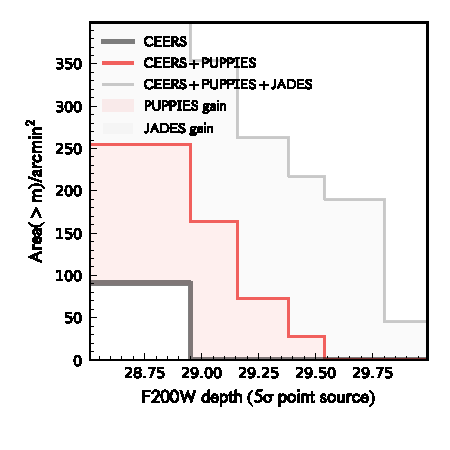
\includegraphics[width=0.3\textwidth]{figs/F200W.pdf}
    \includegraphics[width=0.3\textwidth]{figs/F356W.pdf}
    \caption{The cumulative area probed by WAFLS, JADES, CEERS, and existing \emph{Hubble} and \emph{Spitzer} surveys as a function of the H/F150W-band, F200W, and $3.6\mu$m/F356W (right) depths. \todo{Which is better?}}
    \label{fig:depth}
\end{figure}


\begin{figure}[!h]
    \centering
    \includegraphics[width=0.45\textwidth]{figs/F150W.pdf}
    \includegraphics[width=0.45\textwidth]{figs/F356W.pdf}
    \caption{The cumulative area probed by WAFLS, JADES, CEERS, and existing \emph{Hubble} and \emph{Spitzer} surveys as a function of the H/F150W-band, F200W, and $3.6\mu$m/F356W (right) depths. \todo{Which is better?}}
    \label{fig:depth}
\end{figure}


\begin{SCfigure}
    \includegraphics[width=0.6\textwidth]{figs/F150W.pdf}
      \caption{\protect\rule{0ex}{5ex} TThe cumulative area probed by WAFLS, JADES, CEERS, and existing \emph{Hubble} and \emph{Spitzer} surveys as a function of the H/F150W-band, F200W, and $3.6\mu$m/F356W (right) depths. \todo{Which is better?}}
      \label{fig:depth}
\end{SCfigure}


\noindent
\textbf{Additional constraints} When selecting potential parallel slots we will not only consider potential science duration and background but also the availability of ancillary observations and accessibility to other facilities (e.g. ALMA).

\noindent
\textbf{Alternative Filter Combination Strategies} While all our science objectives can only be fulfilled with all 6 filters a simpler survey utilising only F115W/F150W/F277W/F356W can be used to select $9<z<11$ galaxies and thus constrain the luminosity function, albeit with higher contamination and larger photometric redshift uncertainties. However, such a strategy may be employed particularly for shorter opportunities.

\noindent
\textbf{Alternative read-out mode/$N_{\rm groups}$/$N_{\rm exp}$ strategies} Our fiducial programme assumes both a single exposure for each filter pair in each pointing and adopts the readout mode and number of groups yielding the optimum depth. However each set of observations can be adapted to use different strategies. For example where data volume is a concern the medium tier could instead utilise  \texttt{DEEP8} (with 5 groups) to yield a similar sensitivity.

% \noindent
% \textbf{Alternative read-out/$N_{\rm exp}$ strategies} Because we don't ab initio know the exact configuration of the available parallel observing slots our fiducial visits could be achieved with either one or multiple exposures. In the table below we show several, though not exhaustive, possible configurations for each tier. For example, for the medium tier, while adopting a \texttt{MEDIUM8} readout mode with 10 groups (and a single exposure) yields a slightly more sensitive image, adopting the \texttt{DEEP8} readout mode with 5 groups reduces the data volume considerably. \todo{Is this needed.}

% \begin{center}
% \begin{tabular}{ |l|c|c|c|c|c| } 
%  \hline
% Readout pattern & $N_{\rm groups}$ & $N_{\rm exp}$ & Data Volume/MB & Duration$/s$ & F277W depth ($5\sigma$, AB mag) \\
% \hline
% MEDIUM8 & 5 & 1 & 514 & 515 & 27.63 \\
% SHALLOW4 & 10 & 1 & 942 & 526 & 27.66 \\
% SHALLOW4 & 5 & 2 & 1027 & 515 & 27.55 \\
% \hline
% DEEP8 & 5 & 1 & 514 & 945 & 27.99 \\
% MEDIUM8 & 10 & 1 & 942 & 1052 & 28.03 \\
% MEDIUM8 & 5 & 2 & 1027 & 1031 & 28.02 \\
% SHALLOW4 & 10 & 2 & 1883 & 1052 & 28.04 \\
% SHALLOW4 & 5 & 4 & 2054 & 1031 & 27.94 \\
% \hline
% DEEP8 & 10 & 1 & 942 & 2019 & 28.33 \\
% DEEP8 & 5 & 2 & 1027 & 1890 & 28.37 \\
% MEDIUM8 & 10 & 2 & 1883 & 2104 & 28.42 \\
% MEDIUM8 & 5 & 4 & 2054 & 2061 & 28.41 \\
% \hline
% \end{tabular}
% \end{center}


%%%%%%%%%%%%%%%%%%%%%%%%%%%%%%%%%%%%%%%%%%%%%%%%%%%%%%%%%%%%%%%%%%%%%%%%%%%

%   3. SPECIAL REQUIREMENTS
%        (see https://jwst-docs.stsci.edu/jwst-opportunities-and-policies/jwst-call-for-proposals-for-cycle-1/jwst-cycle-1-proposal-preparation)
%
%
\specialreq             % Do not delete this command.
% Justify your special requirements here, if any.

%%%%%%%%%%%%%%%%%%%%%%%%%%%%%%%%%%%%%%%%%%%%%%%%%%%%%%%%%%%%%%%%%%%%%%%%%%%

%   4. COORDINATED PARALLEL OBSERVATIONS
%        (see https://jwst-docs.stsci.edu/jwst-opportunities-and-policies/jwst-call-for-proposals-for-cycle-1/jwst-cycle-1-proposal-preparation)
%
%
\coordinatedobs % Do not delete this command.
% Enter your coordinated parallel observing plans here, if any.

%%%%%%%%%%%%%%%%%%%%%%%%%%%%%%%%%%%%%%%%%%%%%%%%%%%%%%%%%%%%%%%%%%%%%%%%%%%

%   5. JUSTIFY DUPLICATIONS
%        (see https://jwst-docs.stsci.edu/jwst-opportunities-and-policies/jwst-call-for-proposals-for-cycle-1/jwst-cycle-1-proposal-preparation)
%
%
\duplications           % Do not delete this command.
% Enter your duplication justifications here, if any.

%%%%%%%%%%%%%%%%%%%%%%%%%%%%%%%%%%%%%%%%%%%%%%%%%%%%%%%%%%%%%%%%%%%%%%%%%%%

%   6. ANALYSIS PLAN
%       (see https://jwst-docs.stsci.edu/jwst-opportunities-and-policies/jwst-call-for-proposals-for-cycle-1/jwst-cycle-1-proposal-preparation)
%
%
\analysisplan % Do not delete this command.
% Describe the data processing and analysis plan here.

%%%%%%%%%%%%%%%%%%%%%%%%%%%%%%%%%%%%%%%%%%%%%%%%%%%%%%%%%%%%%%%%%%%%%%%%%%%

\clearpage

\bibliography{WAFLS,WAFLS_quiescent}


\end{document}          % End of proposal. Do not delete this line.
                        % Everything after this command is ignored.
